% TEMPLATE for Usenix papers, specifically to meet requirements of
%  USENIX '05
% originally a template for producing IEEE-format articles using LaTeX.
%   written by Matthew Ward, CS Department, Worcester Polytechnic Institute.
% adapted by David Beazley for his excellent SWIG paper in Proceedings,
%   Tcl 96
% turned into a smartass generic template by De Clarke, with thanks to
%   both the above pioneers
% use at your own risk.  Complaints to /dev/null.
% make it two column with no page numbering, default is 10 point

% Munged by Fred Douglis <douglis@research.att.com> 10/97 to separate
% the .sty file from the LaTeX source template, so that people can
% more easily include the .sty file into an existing document.  Also
% changed to more closely follow the style guidelines as represented
% by the Word sample file. 

% Note that since 2010, USENIX does not require endnotes. If you want
% foot of page notes, don't include the endnotes package in the 
% usepackage command, below.

\documentclass[letterpaper,twocolumn,10pt]{article}
\usepackage{hyperref}
\usepackage{amsmath}

\usepackage{usenix,epsfig,endnotes}
\begin{document}

%don't want date printed
\date{}

%make title bold and 14 pt font (Latex default is non-bold, 16 pt)
\title{\Large \bf Particle-filter based Simultaneous Localization And Mapping (SLAM)}

\author{
{\rm Yiren Lu}\\
GRASP Lab, University of Pennsylvania\\
Mar 2016
}

\maketitle

% Use the following at camera-ready time to suppress page numbers.
% Comment it out when you first submit the paper for review.
\thispagestyle{empty}


\section{Introduction}

In ESE 650 4th project, we did simultaneous localization and mapping (SLAM) of humanoid robot THOR based on Monte Carlo particle filter algorithm ~\cite{thrun2001robust}.
\\
\begin{center}
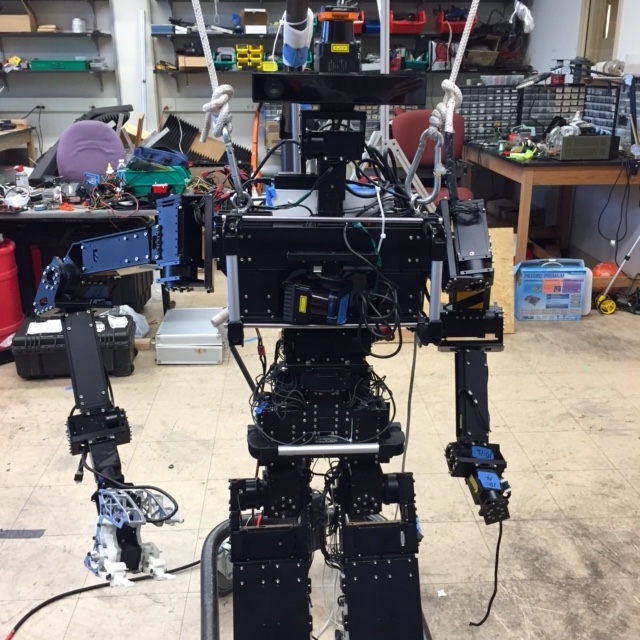
\includegraphics[scale=0.35]{imgs/robot.JPG}\\
\end{center}

\section{Dataset and Preprocessing}

We have data from multiple sensors: Encoder's odometry data, IMU, Kinect, Lidar. In this project, I first simulate the robot path according to the robot's odometry data. Since the encoder's yaw data is less accurate than IMU's yaw, I adopted IMU's yaw and recomputed the incremental motion data. The map reconstructed from the odometry data with IMU's yaw works reasonably well. I also tried compensate head yaw and pitch. For train set 3, adding head's yaw effectively improve the performance. Head's pitch angle does not influence the performance too much. The following is the result only using the odometry data for test set\\

\begin{center}

\includegraphics[width=0.4\textwidth]{results/test_odometry.jpg}
\end{center}


\section{Occupancy Grid Mapping~\cite{thrun2002robotic}}
The occupancy grid is a map representing the belief of whether the position $x,y$ is occupied or free  $m_{x,y}$ by accumulating the measurement($z = {1,-1}$)'s log-odd as follows:\\
\begin{center}
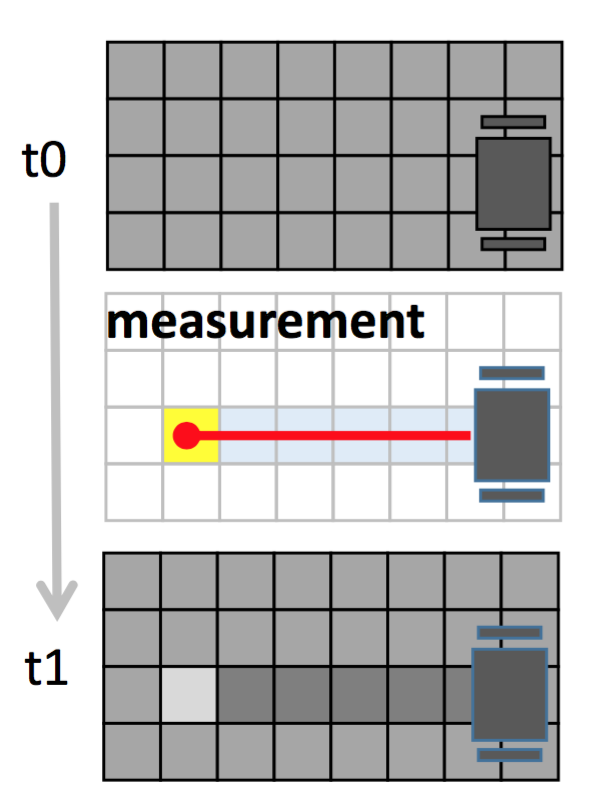
\includegraphics[width=0.25\textwidth]{imgs/lidar}
\end{center}

\begin{align*}
\mbox{logodd} =& log\frac{p(z|m_{x,y}=1)p(m_{x,y}=1)}{p(z|m_{x,y}=0)p(m_{x,y}=0)}\\
=& log\frac{p(z|m_{x,y}=1)}{p(z|m_{x,y}=0)}+log\frac{p(m_{x,y}=1)}{p(m_{x,y}=0)}\\
\\
\mbox{logodd}_{occ}=& log\frac{p(z=1|m_{x,y}=1)}{p(z=1|m_{x,y}=0)}\\
\mbox{logodd}_{free}= & log\frac{p(z=-1|m_{x,y}=0)}{p(z=-1|m_{x,y}=1)}\\
\\
logodd =& \begin{cases} logodd+logodd_{occ}, & \mbox{if } \mbox{ z=1} \\ logodd+logodd_{free}, & \mbox{if } \mbox{ z = -1} \end{cases}  
\end{align*}

\section{Particle Filter based Localization}
I implemented Monte Carlo particle filter for robot localization. The procedure is:
\begin{itemize}
\item Initialize $N$ particles
\item For each timestamp, process the particles with odometry data and add noise
\item Comparing map correlation and reweight the particles according to their correlation level to the existing map
\item Calculate effectiveness factor $Neff = \frac{(\sum_i w_i)^2}{\sum_i w_i^2}$, if it's less than $\alpha N$, then resample according to importance. For my implementation, $\alpha = 0.7$
\item Collect sensor's data, do mapping using the particle with largest weights
\item Repeat
\end{itemize}
\section{Ground Detection}
I implemented Random sample consensus (RANSAC) algorithm to fit ground plane. However in this project, there is an easier way. Here is the depth image to position $(x,y,z)$ mapping:\\
\begin{center}
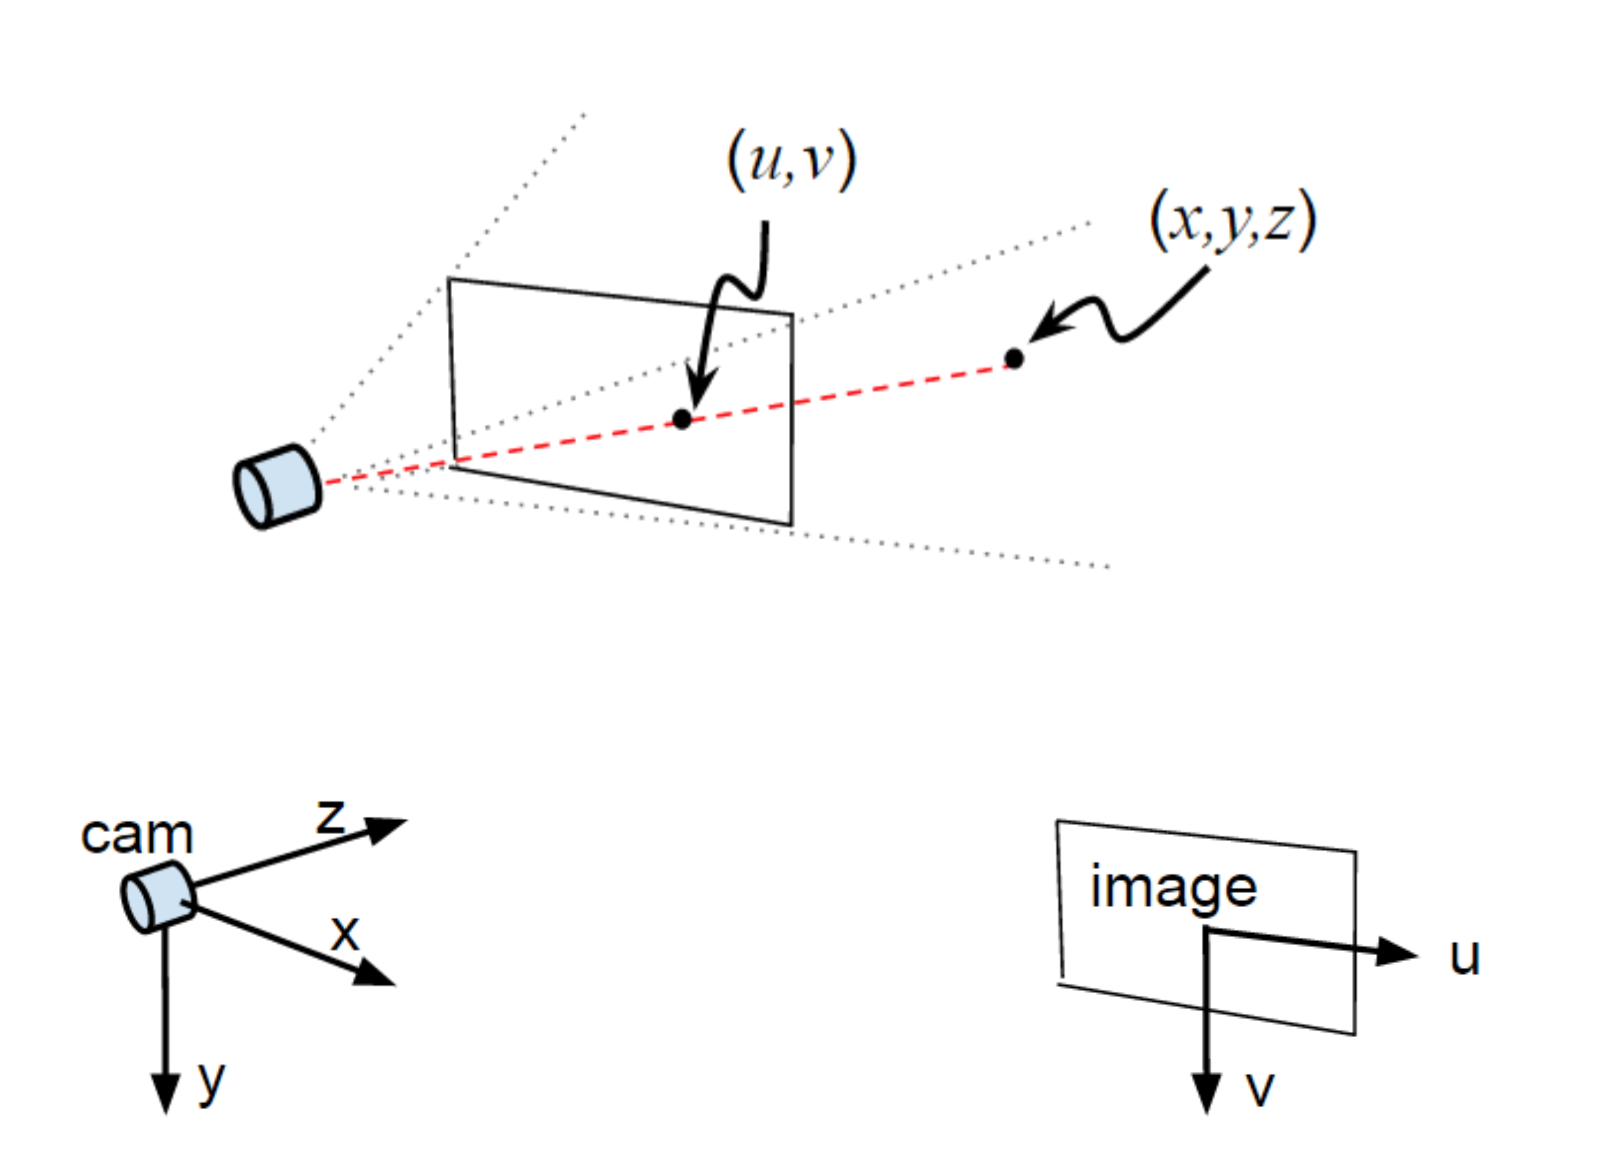
\includegraphics[width=0.35\textwidth]{imgs/cam}
\end{center}
\begin{align*}
\frac{u}{f_u} = \frac{x}{z} \\
\frac{v}{f_v} = \frac{y}{z}
\end{align*}
A ground point should simply satisfies:\\
\begin{align*}
\big| \frac{v}{f_v} - \frac{h}{z}\big| < \epsilon
\end{align*}
Where, h is the height of camera and epsilon is the threshold.
\section{Results and Discussion}

\begin{itemize}
\item I tuned my parameters a lot but here is the best results I have currently as shown in the following images. Due to time limitation, I haven't finished the RGB mapping yet.
\item Surprisingly, on the test set, the map reconstruction from odometry data is slightly better than with particle filter. 
\end{itemize}

\begin{figure}[h]
    \centering
    
\includegraphics[width=0.5\textwidth]{results/train0.jpg}
    \caption{Train set 0}
    \label{fig:train0}
\end{figure}
\begin{figure}[h]
    \centering
    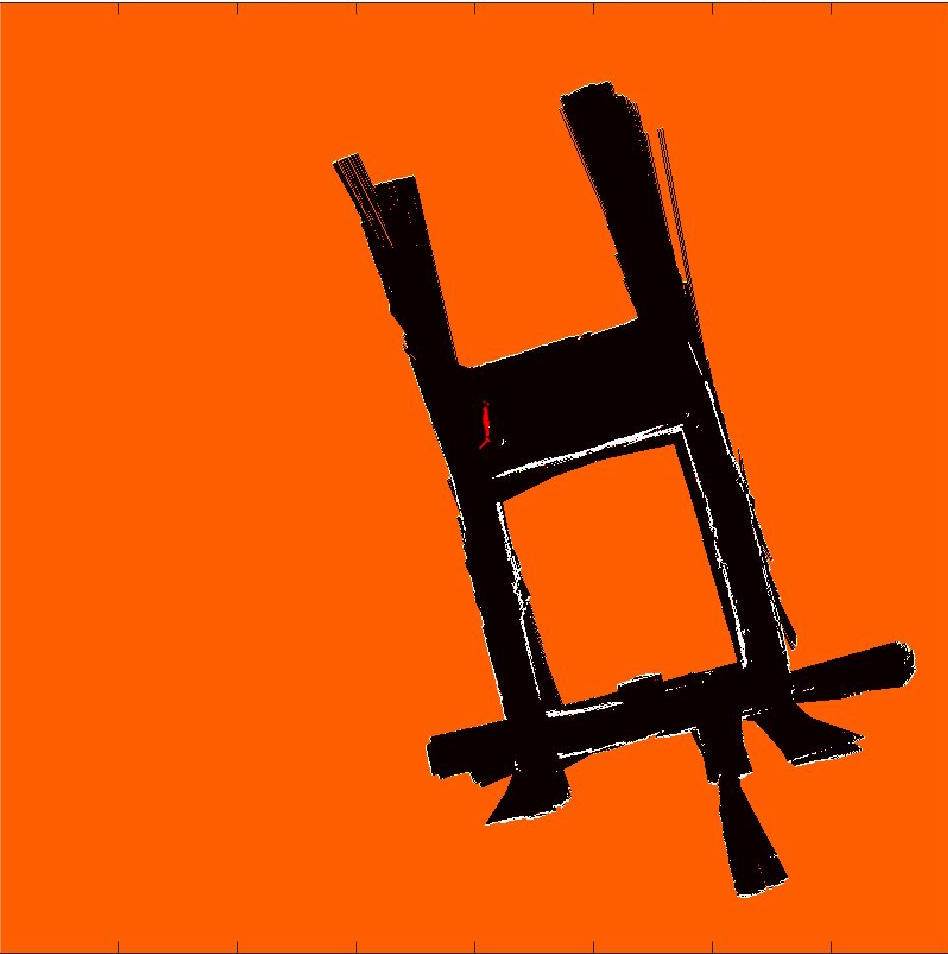
\includegraphics[width=0.5\textwidth]{results/train1.jpg}
    \caption{Train set 1}
    \label{fig:train1}
\end{figure}
\begin{figure}[h]
    \centering
    
\includegraphics[width=0.5\textwidth]{results/train2.jpg}
    \caption{Train set 2}
    \label{fig:train2}
\end{figure}
\begin{figure}[h]
    \centering
    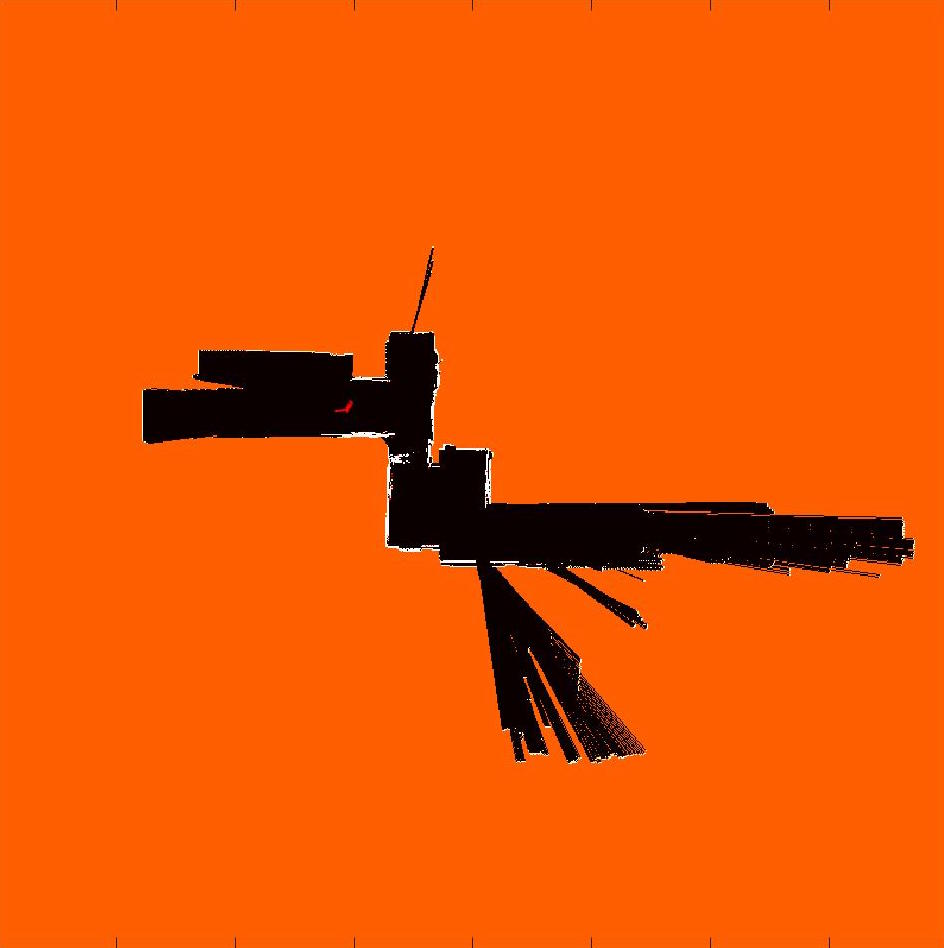
\includegraphics[width=0.5\textwidth]{results/train3.jpg}
    \caption{Train set 3}
    \label{fig:train3}
\end{figure}
\begin{figure}[h]
    \centering
    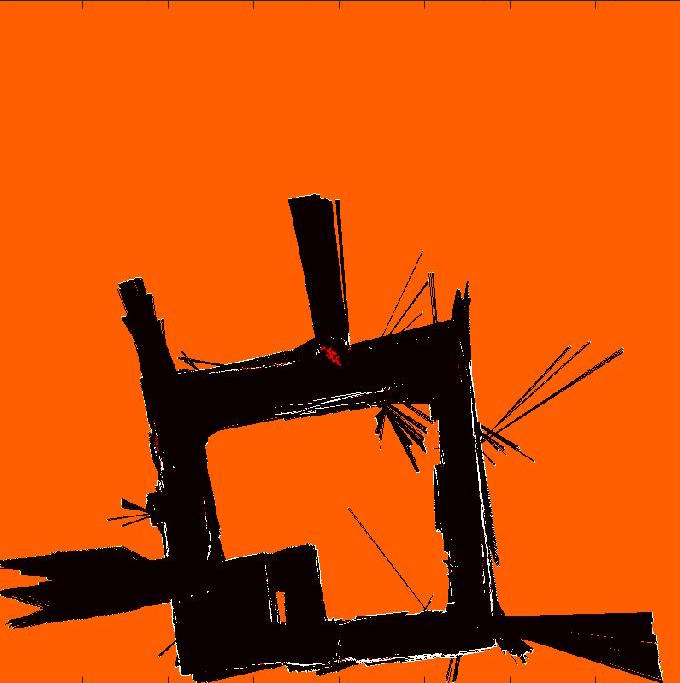
\includegraphics[width=0.5\textwidth]{results/test.jpg}
    \caption{Test set}
    \label{fig:test}
\end{figure}
\begin{figure}[h]
    \centering
    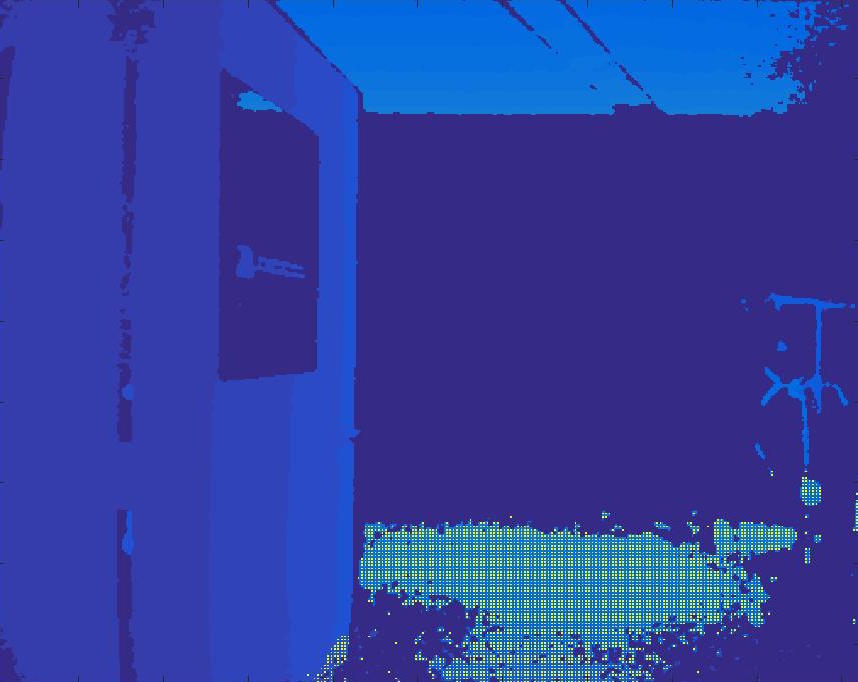
\includegraphics[width=0.5\textwidth]{results/train0_ground_d.jpg}
    \caption{Ground detection for train set 0}
    \label{fig:ground0}
\end{figure}
\begin{figure}[h]
    \centering
    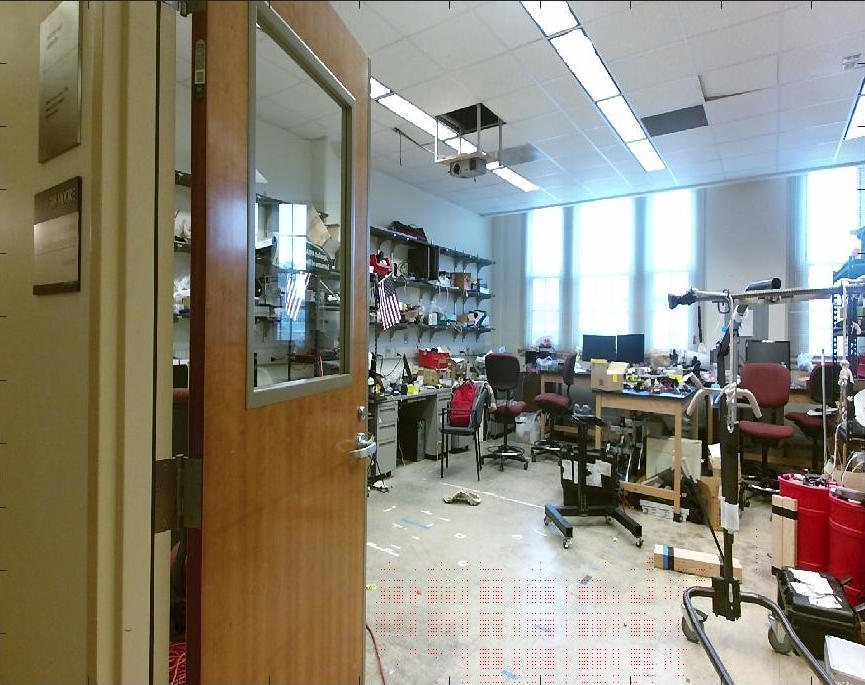
\includegraphics[width=0.5\textwidth]{results/train0_ground_rgb.jpg}
    \caption{Ground detection for train set 0 mapping to rgb image}
    \label{fig:ground0rgb}
\end{figure}

\begin{figure}[h]
    \centering
    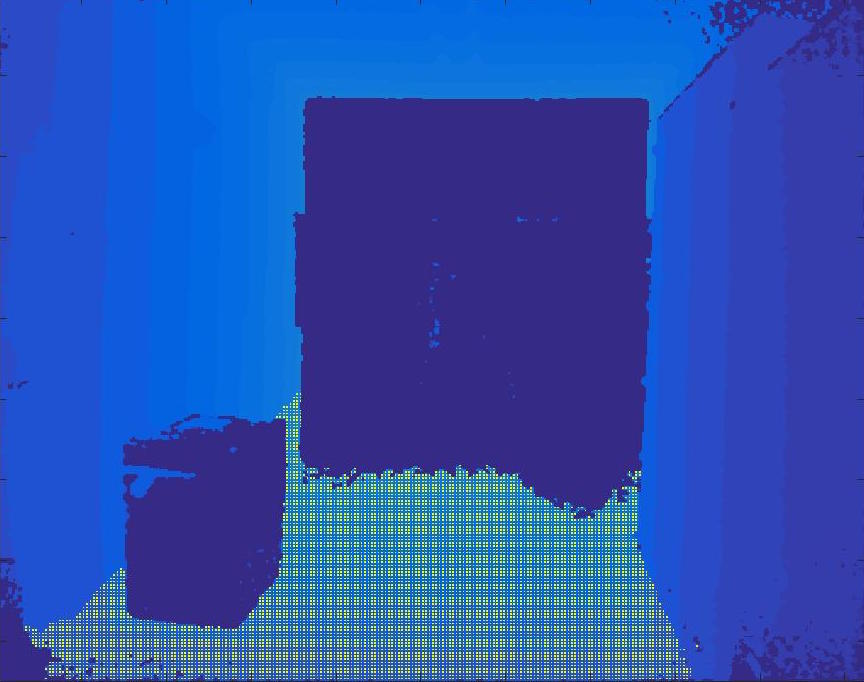
\includegraphics[width=0.5\textwidth]{results/test_ground_d.jpg}
    \caption{Ground detection for test set}
    \label{fig:ground0}
\end{figure}



\section*{Acknowledgement}
Thanks Dr. Lee for designing and preparing this project and thanks TAs for timely responses to our questions.

{\footnotesize \bibliographystyle{acm}
\bibliography{sample}}


% \theendnotes

\end{document}







